\documentclass[a4paper,10pt]{article}
\usepackage{graphicx}
\usepackage{amsfonts}
\usepackage{amssymb}
\usepackage{amsmath}
\usepackage{latexsym}
\usepackage{enumerate}
\usepackage{mdwlist}
% Set some parameters to make the document look better.
\setlength{\parskip}{0.25pc}
%\setlength{\parindent}{0pt}
%opening
%\title{An Exploration of HQSOMs}
\title{An Exploration of Hierarchical Quilted Self-Organizing Maps}
\author{Theodore Hilk, Joseph Lynch}
\begin{document}

\maketitle

\begin{abstract}
\noindent We explore the paper ``Biomimetic sensory abstraction using hierarchical quilted
self-organizing maps," by J. W. Miller and P. H. Lommel of the Charles Stark Draper Laboratory. We
place the paper in historical context, provide a high-level summary, and briefly review related
literature. We give both a qualitative overview and a specific mathematical formulation of the
hierarchical quilted self-organizing map (HQSOM) model, and provide a thorough, reproducible record
of our design and implementation process for a Python-based HQSOM framework. We present our results
from conducting each of the experiments described in Miller and Lommel's paper, which involved the
classification of various shapes invariant to shift and scale transformations in 3x3- and 7x7-pixel
fields. We obtain results consistent with those of the authors, albeit noting considerable
dependence on parameter values and the ambiguity of a certain key formula in the paper.
Subsequently, we develop and test several improvements to the HQSOM algorithm itself.  Some
result in outperforming the original in classification tasks, especially when noise is introduced.
We then implement preprocessing adaptations to allow us to apply both the original and improved
HQSOM algorithms to audio, and we succeed in developing a genre classifier with excellent
out-of-sample performance. We conclude by describing further possibilities for extension and
discussing the broader significance of this line of research.
\end{abstract}
\section{Introduction and Motivation}

Biologically-motivated algorithms have a long history in artificial intelligence and machine
learning. Indeed, AI as a field was born out of attempts to simulate human intelligence using
artificial systems\cite{AIHistory1}, and one of the earliest techniques, the perceptron, was
explicitly based on a simplified model of a biological neuron.\cite{Rosenblatt}

Although symbolic approaches enjoyed much more prominence following the publication of papers
recognizing the limitations of early neural networks in the early 1960s\cite{DreyfusMind}, their own
difficulties in dealing with problems of perception, learning, and pattern recognition led to a
resurgence of interest in sub-symbolic systems from the 1980s onward.\cite{AIHistory1, AIHistory2,
MLHistory1} It was during this period that the field of machine learning gained substantial
prominence, focusing on pattern recognition, classification, and adaptive control, and placing a
heavy emphasis on quantitative and often statistical methods as opposed to symbolic and logical
ones.\cite{MLHistory1}

Beginning largely in the early 1990s, collaboration in turn between machine learning researchers and
neuroscientists produced models of neurological and cognitive systems demonstrating both strong
concordance with empirical observations and excellent performance in the tasks addressed by those
same systems.\cite{Poggio} Investigation in the area from that time onward has focused on the theory
and simulation of increasingly substantial and complex aspects of human neuroscience, with a
particular emphasis on neocortical functionality, the problem of vision, and the use of
hierarchical, invariant representations for sensory stimuli.\cite{Poggio, HQSOM} The significance of
such modeling efforts can hardly be overstated: they have led to new findings in neuroscience,
improvements in brain-computer interface technology, and perhaps most profoundly, a new paradigm in
artificial intelligence research.\cite{HQSOM, OnIntelligence}

Currently, the most prominent of these models include the Neocognitron (Fukushima), HMAX
(Riesenhuber, Poggio, Serre), the Neural Abstraction Pyramid (Behnke), Hierarchical-Temporal Memory
(HTM) (George, Hawkins), Adaptive Resonance Theory (Carpenter, Grossberg), and VisNet (Stringer,
Rolls).\cite{HQSOM} With the exception of HTM, each of these approaches either relies on substantial
hard-coded \em a priori \em knowledge specific to vision, neglects the role of temporal associations
in learning, or requires separate training and execution phases in use.\cite{HQSOM, HTMAlgo} HTM in
turn involves complex and inelegant models of ``neurons", though they bear little resemblence to
those modeled by computational biologists, and at its core is nothing more than a recurrent
spatio-temporal clustering algorithm incorporating interlayer feedback to provide auto-associative
prediction capabilities.\cite{HTMAlgo}

Our goals in undertaking this project were to identify and generalize the essential aspects of
existing hierarchical cortical models, and to extend and improve upon techniques from the
literature. Therefore, we chose the simplest and most general such model we could find that was not
subject to the above-enumerated limitations. This was the Hierarchical Quilted Self-Organizing Map
(HQSOM) model developed by Miller and Lommel, which we have succeeded in analyzing, reproducing,
testing, improving, and extending. 

Specifically, we have implemented the HQSOM model in numerical Python, conducted the same visual
shape recognition experiments as the paper's authors over a wide range of parameter values, and
succeeded in reproducing their results in spite of ambiguity surrounding a particular key formula in
the paper. Further, we have characterized the significance and implications of the HQSOM's
parameters, improved the noise performance of the algorithm by including a mean-squared-error-based
activation function, and enhanced its separability characteristics by using a peripherally
inhibitory "Mexican hat" neighborhood function instead of the standard gaussian.  We have also
improved its convergence rate without
compromising representation quality, through the incorporation of an adaptive learning rate that is
applied to the best-matching input
prototype when a given input differs greatly from all current prototypical
representations.  We have also improved the efficiency of the training process by
creating a "reset" function, which both eliminates the need for blank input sequences between
successive training sequences, and ensures that no residual effects can carry over between these
training sequences. Finally, we have extended our implementation to represent and classify
audio, and successfully built a system to learn and classify music based on genre which performs
very well out-of-sample. We believe that even greater potential exists for the improvement and
generalization of this approach, and we highlight some of our views on the matter in our conclusion
below.

\section{Paper and Summary}

We chose to replicate the paper ``Biomimetic sensory abstraction using hierarchical quilted
self-organizing maps," by Jeffrey W. Miller and Peter H. Lommel of the Draper Laboratory. The paper
develops a novel classification algorithm called a hierarchical quilted self-organizing map (HQSOM),
then applies it to two simple visual processing tasks. The motivation for this approach lies in the
desire to model the operation of the human visual cortex in a way that improves upon the realism of
earlier techniques by: relying more on learning and less on hard-coded \em a priori \em knowledge,
using temporal associations and not just spatial ones to construct representations, and learning
on-line instead of requiring a separate training period.

The paper discusses several benefits of modeling the brain, noting that more accurate models have
allowed for the creation of improved AI techniques, neurophysiological discoveries, and even better
brain-computer interfaces. The authors choose to focus on vision in particular because it has such
rich applications in software and is handled so easily by animals.

They then discuss various aspects of brain structure and function, noting that the isocortex,
comprising about 85\% of the brain in humans, is responsible most sensory processing, motor control,
language, logic, mathematics, and spatial visualization. In spite of this, it appears to have a
uniform, hierarchical structure throughout its various functional regions, and a substantial portion
of the contemporary cognitive neuroscience community posits that the elements of this structure
perform essentially the same information processing operations throughout the cortex.

Examining the ventral stream of the visual cortex in particular, the authors note that its regions
are wired in a hierarchy. At the base, V1 neurons respond to small lines of various orientations in
their respective and narrow portions of the visual field, while neurons in the higher V2 region
respond to somewhat less localized simple shapes, those of the even higher V4 region respond to more
complex shapes across larger areas, and those in the IT region respond invariantly to complex
objects throughout the entire field of view. The authors then mention a few similar cortical models,
noting the above limitations in realism. Such alternative models are described in more detail in our
literature review below.

Miller and Lommel define the goals for their own model in terms of biological functional
equivalence, generalizability across multiple sensory domains, and simplicity. They specifically
note that computational efficiency was only a secondary goal. In pursuing functional equivalence,
the authors take the explicit position that there exists some basic "building block" or unit of the
cortex beyond which no further details must be modeled, so long as the abstract functionality of the
unit is properly preserved.

They describe this functionality in terms of the unsupervised learning of abstract patterns in the
input data, and of the recurrent learning of patterns in the sequences of inputs patterns at lower
levels of the hierarchy. They propose that this reduction of sensory input to abstract concepts may
be conceived in terms of the related processes of spatial and temporal clustering, or "pooling".
Spatial pooling learns patterns of input data that are spatially co-incident at a given level of the
hierarchy, while temporal pooling learns patterns that tend to occur near one another in time.

The authors note that numerous algorithms exist for spatial clustering, including K-means, SOMs,
expectation maximization, winner-take-all neural networks. This is discussed further below in terms
of our current and future extensions to the HQSOM model. Likewise, temporal clustering and sequence
processing can be performed with anything from basic statistical techniques like ARMA, ARIMA, NARMA,
GARCH, N-GARCH, etc. to recurrent neural networks, temporal Kohonen maps (TKMs), or the simpler and
faster-converging recurrent self-organizing maps (RSOMs).

In keeping with this approach, the HQSOM algorithm creates invariant, low-dimensional
representations of high-dimensional data by passing them through successive stages of spatial and
temporal pooling. Spatial pooling is accomplished by means of self-organizing maps (SOMs), while
temporal pooling is handled by a type of modified SOM called a recurrent self-organizing map (RSOM).
The authors elected to use the SOM model because it was familiar to them, and because it is
relatively simple and well-researched. Likewise, they chose RSOMs for temporal pooling due to their
demonstrated performance in the area and their elegant similarity to the ordinary SOM.

A SOM, or Kohonen network, is a type of unsupervised nonlinear dimensionality reduction algorithm,
often used for data visualization. It can also be viewed as a form of vector quantization. SOMs
operate by building a table of "weight vectors" in the input space, then modifying the weight
vectors closest to each successive input vector to make them closer to that input vector, such that
the set of weight vectors overall converges to yield a summary representation of the clusters in the
input data in a topology-preserving fashion. An RSOM is a SOM that takes an exponential moving
average over the differences between input vectors and weight vectors when computing these
distances, which allows measures of similarity to extend across a succession of inputs and hence
into the temporal domain. Both SOMs and RSOMs are described in more mathematical detail in the
section entitled \em System Design and Variables \em below.

After describing the motivation and technical details of HQSOMs, Miller and Lommel's paper describes
the recursive combination of HQSOM base units, which are comprised of a SOM whose regularized
activation vector over its weight vectors is provided as input to an RSOM (see below for specific
mathematical details). The SOM performs spatial clustering over its input, yielding a set of
representative spatial feature vectors in the input space, and the RSOM proceeds to perform temporal
clustering over sequences of these spatial patterns, such that the RSOM's weight vectors each
correspond to some particular spatiotemporal cluster in the input data. Thus, the HQSOM base unit as
a whole produces a dimensionally-reduced representations of the spatiotemporal contents of its
input. It produces spatiotemporal abstractions. Composing HQSOMs in a hierarchical arrangement, such
that the activation vector over the weight vectors of the RSOM in a given HQSOM base unit are
provided as the inputs to the SOM of another HQSOM base unit, allows for the representation of
progressively more invariant spatiotemporal patterns in the input data.

The authors then describe two experiments involving the learning and classification of simple visual
patterns, which we describe in detail and reproduce below.

\section{Hypothesis, Plan, and Risks}
We wish to begin by re-implementing the HQSOM algorithm described in the paper, using numerical
Python.  The primary risk in doing so is that the algorithm is rather complex, and certain aspects
are not thoroughly described.  We also expect that it will take a long time to code, and that the
high dimensionality and fairly opaque nature of the HQSOM's representations may make it difficult to
debug our implementation.  For example, if a network is failing to produce the desired result,
looking at the RSOM unit map is not particularly helpful.

We will then attempt to reproduce the experimental results presented by Miller and Lommel,
which showed that HQSOMs could form shift- and scale-invariant representations of various shapes
within
3x3- and 7x7-pixel fields of vision.  We expect that the testing framework and test data may take a
considerable amount of time to create.  We also anticipate that the experimental results may be
difficult to reproduce due to parameter sensitivity, and that computational efficiency may pose
hurdles given the number of training cycles used in the paper.  As above, we again note that it can
be difficult to debug these types of networks due to the internal structure being fairly
mathematical in nature.  Finally, the potential fragility of
these types of systems is well known in the academic community, so it is very possible that we will
not be able to get any viable results whatsoever due to bad parameters and long test runs.

Once we are able to replicate these results to a
reasonable degree of precision, we will extend the HQSOM framework into the audio domain and attempt
to
classify music by genre.  The main risks emerge from the potential complexity of these extensions,
the nuances involved in producing high-quality spectrograms, and the anticipated large size and
computational burden of networks capable of classifying something as abstract as genre.

\section{System Design and Variables}
HQSOM networks are comprised of hierarchically stacked building blocks known as HQSOM base units.
An HQSOM base unit in turn consists of a stacked SOM-RSOM pair, such that input to the base
unit as a whole is provided as the input to the SOM, then the regularized activation vector over the
map space of the SOM is provided
as the input to the RSOM, and finally the activation vector over the map space of the RSOM is
provided as the input to
any HQSOM base units stacked above this one.  If this is the top unit in the network, then this
final RSOM activation vector yields an invariant summary of the input data as a whole and may be
used for classification.
Composing these SOM-RSOM pairs into multi-layered networks yields Hierarchical Quilted
Self-Organizing Maps (HQSOMs), which can
identify both spatial and temporal clustering in data over multiple levels of abstraction.  The
general use case for HQSOMs is to identify spatiotemporal clusters in input data, such that a
supervised learning technique can be applied to actually make the classification, since the clusters
themselves rely on some associated semantic meaning in order to be regarded as labels.  However, for
the sake of this paper, we will take such semantic meaning for granted and thus consider
clustering equivalent to classification. The following
discussion of SOMs, RSOMs and HQSOMs is based on the corresponding sections of the Miller and Lommel
paper, and hence the vast majority of this method explanation can be found in that
paper as well \cite{HQSOM}.
\subsection{SOM}
The basic SOM computational block can either be trained on data or asked to classify data. The SOM
is made up of a $m$x$n$ matrix that maps inputs of dimension $m$ to outputs of dimension $n$.  For
example a SOM designed to take in 3d vectors and output a 5d vector looks like:

\begin{center}
$
\begin{pmatrix}
.3 & .7 & .1  & .14 & .01\\
.3 & .1 & .01 & .16 & .9\\
.3 & .03 & .8 & .7  & .01
\end{pmatrix}
$
\end{center}
Each column is a map unit, and whichever map unit $\bold{w_b}$ is closest to the input $\bold{x}$
is considered the best-matching unit (BMU).  The measure of closeness is usually simply Euclidean
distance, so:
\begin{equation}
 \bold{w_b} = argmin_{w_i} ||\bold{x} - \bold{w_i}||
\end{equation}
 
During the training stage, input vectors are applied to the input and then an
update rule is applied over the entire map space that shifts map units that are nearest to the
input data towards the input data:
\begin{equation} \label{eq:UPDATE}
 \bold{w_{i}}(t+1) = \bold{w_i}(t) + \gamma h_{ib}(t)(\bold{x}(t)-\bold{w_i}(t))
\end{equation}
where gamma is the rate of learning, $h_{ib}$ is the neighborhood function, and $\bold{w_i}$ is the
map unit being modified.  The neighborhood function is defined as a function that is close to zero
for units far away from the BMU.  Traditionally a Gaussian is used:
\begin{equation} \label{eq:GAUSSIAN}
 h_{ib}(t) = exp(\frac{-||I_i-I_b||^2}{\mu(t)\sigma^2})
\end{equation}
where $I_i$ indicates the index of the $i$th unit, $\mu(t)$ is a decreasing function of mean
squared error and $\sigma$ is the learning radius.  A SOM therefore has two parameters that need to
be tuned: the learning rate $\gamma$ and the learning radius $\sigma$. For example, two sample unit
maps after an update with $\bold{x}=(.1,.1,.1), \gamma=.2$ and different sigmas would look like:
\begin{figure}[h]
\begin{center}
$
\begin{pmatrix}
0.26 &  0.7 &  0.1 &  0.14  & 0.01 \\
0.26  & 0.1  & 0.01 & 0.16 & 0.9  \\
0.26  & 0.03 & 0.8  & 0.7  & 0.01
\end{pmatrix}$
\caption{$\sigma$ = 1}
\centering
$\begin{pmatrix}
0.26 &  0.607 &  0.1 &  0.139  & 0.01 \\
0.26  & 0.1  & 0.017 & 0.159 & 0.897  \\
0.26  & 0.041 & 0.748  & 0.687  & 0.01
\end{pmatrix}
$
\caption{$\sigma$ = 100}
\end{center}
\end{figure}
Clearly, the update with the larger sigma affected more of the map space.  Also it is important to
note that units were pulled towards the input, but with a less dramatic effect as the map index
increased (separating itself further from the BMU).

During activation, the SOM can return two types of activation vectors:
\begin{enumerate}
\item Discrete: A vector of the correct dimension with the BMU index set to 1 and all others set
to 0.
\item Continuous: A vector $A(t)$ defined as the normalized form of a vector constructed as follows:
\begin{equation}
 A_i = \frac{1}{||\bold{x(t)} - \bold{w_i}||^2}
\end{equation}
\end{enumerate}


\subsection{RSOM}
The Recurrent SOM is an extension of the basic SOM that adds an exponential moving average of
differences between observed inputs and units in the map with time-decay parameter $\alpha$ . At
each update the differences are updated and instead of looking for the BMU in map space, the BMU
index is chosen by finding the minimum magnitude recursive difference. Furthermore, instead of
applying $\bold{x}(t)$ directly to the map, the recursive difference for a particular unit is
applied in each unit's update rule and $\bold{x}(t)$ is used to update the recursive difference
matrix:
\begin{equation}
 \bold{y_i}(t+1) = (1-\alpha)\bold{y_i}(t)+\alpha(\bold{x}(t)-\bold{w_i}(t))
\end{equation}
The update rule becomes:
 \begin{equation} \label{eq:RUPDATE}
 \bold{w_{i}}(t+1) = \bold{w_i}(t) + \gamma h_{ib_r}(t)\bold{y(t)}
\end{equation}
where the neighborhood function is computed using the recursive BMU as the BMU index instead of the
map space BMU.  The proper tuning of $\alpha$ depends on how responsive one wishes for the RSOM to
be: lower values of $\alpha$ cause the moving average of inputs to dominate (long term memory),
whereas higher values of $\alpha$ (close to 1) mean that recent inputs dominate (short term memory)

\subsection{SOM-RSOM Pair}
The final computational structure is the SOM-RSOM pair.  Recognizing that SOMs are effective at
identifying spatial clustering, and RSOMs are effective at identifying temporal clustering, but
SOMs do zero temporal clustering and RSOMs have degraded spatial clustering, the SOM-RSOM pair is
intended to get the best effect of both.  First the input data is fed into the SOM to get a spatial
representation, and then this representation is fed into the RSOM to do temporal clustering. 
\section{Implementation Process and Results}
Two implementations of SOMs and RSOMs were written, one being as close as possible
to the reference implementation for reproducibility, and the other having a number of slight
changes to improve convergance.  As is to be expected, the reference paper leaves out a
number of implementation details so this is our best approximation.
\subsection{Reference Implementation of SOM and RSOM Units}
Self-Organizing Maps were implemented via a Python class with three main methods: a constructor,
an update method that takes a numpy array representing the input vector as well as the learning
parameters (gamma, sigma, etc...) to use for that particular update and modifies the internal state
of the SOM accordingly, and a method to request the activation vector for a given input vector.
Internally the SOM map was stored
as a $m$x$n$ numpy array where $n$ is the input vector size and $m$ is the size of the map space. 
During an update call, the Best Matching Map Unit (BMU) for any given input vector was determined
using a linear search for the minimum Euclidean distance and then all map units near to the BMU as
well as the BMU were shifted towards the input according to a Gaussian neighborhood function.  The
standard SOM update rule was used as per equation ($\ref{eq:UPDATE}$).
 
A linear search was prefered due to the high dimensionality of the space, and a Gaussian
neighborhood function was chosen for reproduceability.  The activation method returned either a
discrete or a continuous representation of the map's activation to a given input. The discrete
representation is defined as above, and the normal representation is given in equation
($\ref{eq:EUCMETH}$) where $a_i$ represents the $i$th position in the activation vector,
$\bold{w_b}$ is the BMU, $\bold{x}$ is the input vector, and $\bold{w_i}$ represents the $i$th map
unit.
\begin{equation} \label{eq:EUCMETH}
 a_i = \frac{1}{||\bold{w_i}-\bold{x}||}, \bold{a} = \frac{\bold{a}}{||\bold{a}||}
\end{equation}
\\
Recurrent Self-Organizing Maps were simply a subclass of the SOM that use the modified RSOM update
rule as well as storing the recursive difference matrix as a numpy array.  The time decay parameter
($\alpha$) was passed in at every update call.

\subsection{Basic Design of SOM-RSOM Pair and Other Hierarchical Structures}
Since both SOMs and RSOMs are implemented as Python objects, the SOM-RSOM pair simply consisted of
a SOM object and a RSOM object with an update and activation method that takes in an input vector
$\bold{x}$, feeds it into the SOM to get a transformed activation vector $\bold{y}$ and finally
takes that $\bold{y}$ and feeds it into the RSOM to get the final output which is the BMU of the
RSOM.  The only difference between the SOM-RSOM update and activation methods is that the update
method calls update internally (thus changing the state of the network), whereas the activation
method merely passes along activation
vectors. In the code this SOM-RSOM pair was refered to as a HQSOM because a single SOM-RSOM pair
does indeed form the simplest HQSOM.

Hierarchies were built at first by hard wiring these HQSOM base units together.  However, in order
to facilitate testing of the audio extension, a framework was designed that allowed for any
arbitrary tree HQSOM accepting input with a 1-dimensional topology (e.g. a line of pixels or
spectral power densities, as opposed to a 2d image).  The first level of the tree reads data from
the input, and passes its activation vector to the next layer, which passes its activation vector to
the next layer, etc ...  The output of the top level node is the representation of the input that is
(hopefully) invariant under certain conditions.

\subsection{Replication of First Experiment}
The first experiment presented in the paper was a simple example of 3x3 images with 3
pixel horizontal and vertical lines that have been shifted to all possible positions.  This data
set is small enough to be enumerated, and simple enough in concept to use a single SOM-RSOM pair as
the HQSOM network.  We implemented the network as a single HQSOM that had an input size of 9,
internal SOM map size of 18, and internal RSOM map size of 3.  We mapped the 3x3 image grids
to a linear vector of size 9 by iterating through the image left to right and top to bottom.
The mapping used is shown in Figure $\ref{fig:3TestMapping}$.
\begin{figure}[ht]
\begin{center} 
$\begin{pmatrix}
1 & 2 & 3 \\
4 & 5 & 6 \\
7 & 8 & 9 
\end{pmatrix}
\rightarrow
\begin{pmatrix}
1 & 2 & 3 & 4 & 5 & 6 & 7 & 8 & 9 
\end{pmatrix}
$
\end{center} 
\caption{Experiment 1 Image to Vector Mapping}
\label{fig:3TestMapping}
\end{figure} 

The implementation was shown to be correct by two different tests: performance on non-noisy
data, and aggregate performance over many noisy data sets. During training, the HQSOM is exposed to
three blank images, followed by three line images, followed by three blank images where the three
line images alternate between the three horizontal and the three vertical images. An example
training sequence (without noise) is shown in Figure $\ref{fig:3TestData}$.
\begin{figure}[ht]
\begin{center} 
 \includegraphics[scale=.3]{./exp1_dataset.png}
 % exp1_dataset.png: 200x200 pixel, 72dpi, 7.05x7.05 cm, bb=0 0 200 200
\end{center} 
\caption{Experiment 1 Training Sequence}
\label{fig:3TestData}
\end{figure} 
Applying the sequence shown in Figure $\ref{fig:3TestData}$ hundreds of times with parameters
$\gamma_{som} = \gamma_{rsom} = .1, \sigma_{som}=16, \sigma_{rsom}=90,$ and $ \alpha = .1$
trained the HQSOM and clustered the weight vectors in the map units of the SOM and RSOM. Since the
blank images are solely meant to reset the RSOM EMA difference matrix, a method was added to RSOMs
and HQSOMs that allows the difference matrix to be cleared (with a random index selected to have a
value of .01 so that the BMU varies randomly after each reset) and the training steps with blank
images were replaced with a call to this function. After roughly 2500 training samples were shown to
the network, the HQSOM was asked to classify (return the BMU of the top level RSOM) each piece of
data again and as expected all horizontal lines were classified the same, all vertical Lines were
classified the same, and all blank images were classified the same regardless of position.  The
network had successfully formed an invariant representation of vertical and horizontal lines in a
3x3 field of view.
\\
To test the noise tolerance of the network, Gaussian noise with standard deviation .1, .2, .25 and
.3 was applied to the test data, which was then trained on as before and the HQSOM was again asked
to classify samples of noisy vertical and horizontal lines (with different noise from the training
data).  The results of 100 trials with each noise level are summarized in the following table:
\begin{center}
  \begin{tabular}{ | c | c | c | }
    \hline
    Noise Std. Deviation & Number Correctly Clustered\\ \hline
    .1 & 99/100 \\ \hline
    .2 & 31/100 \\ \hline
    .25 & 5/100 \\ \hline
    .3 &  4/100\\
    \hline
  \end{tabular}
\label{table:3TestResults}
\end{center}
Clustering ``correctly'' simply means that all vertical lines had the same BMU at the output, all
horizontal lines had the same BMU at the output but different from the vertical lines, and all
blank images had the same BMU at the output but different from either the vertical or horizontal
lines.  For example: $ \begin{pmatrix} 1 & 0 & 0 & 0 & 2 & 2 & 2 \end{pmatrix}$ is a ``correct''
clustering if we apply one blank image, three vertical lines, and three horizontal lines but $
\begin{pmatrix}  2 & 0 & 0 & 0 & 0 & 0 & 0 \end{pmatrix}$ is not. It is worth noting that when fewer
than 2000 training steps were taken the map would often converge to a ``Something vs Nothing'' map
in that the HQSOM would be very good at clustering lines together and blank images together, but
would not differentiate between the two types of lines.  This makes sense because the alpha is
small enough that it could take time for the final representation to form.

\subsection{Replication of Second Experiment}
The second experiment presented in the paper aimed to create shift and scale invariant
representations of squares, diamonds, and X shapes in a 7x7 grid.  To replicate this experiment, a
two tiered network was created such that there were 9 low level HQSOMs that each inspected a 3x3
swatch of the 7x7 grid with 1 pixel overlaps on each side.  These base units fed into a top level
HQSOM having a 9 dimensional vector input (composed of the BMUs of each of the bottom level HQSOMs),
which in turn
outputted a BMU index representing the cluster an input belongs to. The goal was to find a shift
invariant representation of these shapes by exposing the network to each family of shapes that
are both scaled and then shifted around in a spiral fashion, followed by blanks for 100 steps,
and then the next shape, more blanks, and so on.  The input sequence is shown in Figure
$\ref{fig:7TestData}$.
\begin{figure}[ht]
\begin{center}
 \includegraphics[scale=.3]{./exp2_dataset.png}
 % exp2_dataset.png: 813x175 pixel, 72dpi, 28.68x6.17 cm, bb=0 0 813 175
\end{center}
\caption{Experiment 2 Input Data}
\label{fig:7TestData}
\end{figure} 

The paper claims upward of 95\% clustering, but we were unable to even achieve a four
classifier using the specified parameters from the paper as per Figure $\ref{fig:PAPERSPECS}$. 
\begin{figure}[ht] 
 \begin{center}
  \begin{tabular}{ | l | c | c | c | c | }
    \hline
    & $\gamma$ & $\alpha$ & $\sigma$ & Map Size\\ \hline
    Layer 1 SOMs  & .1   & 1   & 4  & 65\\ \hline
    Layer 1 RSOMs & .01  & .1  & 10 & 17\\ \hline
    Layer 2 SOMs  & .1   & 1   & 2  & 513\\ \hline
    Layer 2 RSOMs &  .001 & .01 & 50 & 17 \\
    \hline
  \end{tabular}
\caption{Experiment 2 Parameters}
\label{fig:PAPERSPECS}
\end{center}
\
\end{figure}

The best
run of our HQSOM yielded the following final distribution where the final distribution is simply the
number of test images classified as that BMU divided by the total number of test images for a given
data set.

\begin{center}
\small
\begin{verbatim}
################################################################################
Data Set: BLANK
Most Frequently Classified As (MODE): 4
Full Distribution over Final RSOM Map Space:
[ 0.  0.  0.  0.  1.  0.  0.  0.  0.  0.  0.  0.  0.  0.  0.  0.  0.]
################################################################################
Data Set: SQUARE
Most Frequently Classified As (MODE): 3
Full Distribution over Final RSOM Map Space:
[ 0.          0.08571429  0.17142857  0.45714286  0.28571429  0.          0.
  0.          0.          0.          0.          0.          0.          0.
  0.          0.          0.        ]
################################################################################
Data Set: DIAMOND
Most Frequently Classified As (MODE): 2
Full Distribution over Final RSOM Map Space:
[ 0.          0.14285714  0.77142857  0.08571429  0.          0.          0.
  0.          0.          0.          0.          0.          0.          0.
  0.          0.          0.        ]
################################################################################
Data Set: X
Most Frequently Classified As (MODE): 2
Full Distribution over Final RSOM Map Space:
[ 0.          0.          0.97142857  0.02857143  0.          0.          0.
  0.          0.          0.          0.          0.          0.          0.
  0.          0.          0.        ]

\end{verbatim} 
\end{center}

While there is certainly convergence, it is not 95\%.  Due to the fact that runs of this particular
simulation took well over 9 hours, we were only able to test about 10 different
parameter combinations, none of which yielded a better result then the one supplied above.  It
appeared that the HQSOM was not using the full breadth of the RSOM map space in any of the HQSOM
units, which may have resulted from an incorrect formulation of the activation vectors that were
being passed up.  We suspect this as the cause because the formulas presented in the paper for the
continuous version of the activation vectors were not well-formed.  Thus, we had to deduce the
proper formulas based on somewhat unclear explanations of these vectors and their significance.  It
was also noticed that the networks frequently converged to certain states very quickly
and then never moved from that state.  The lack of a good activation vector and unintentional fast
convergence
led us to the following innovations:
\begin{enumerate}
\item A regularized activation vector based on the Mean Squared Error of the BMU vector.
\item The notion of an adaptive $\gamma$.
\item The use of a Mexican Hat neighborhood function (second derivative of Gaussian) instead of a
Gaussian neighborhood function.
\end{enumerate}
 
\subsection{Changes to Algorithm and Relative Performance}
Having completed the implementation of the paper's networks as far as deemed feasible, the three
innovations previously mentioned were implemented in code and tested to compare relative
performance. In all cases our implementation proved to be superior, especially when we began
testing our Audio extension.
\\
\\
We began by implementing the new activation vector.  Since the adaptive $\sigma$ function was based
on minimizing the mean-squared error (MSE) of the BMU and input vector, we believed that it would
also be a good metric to measure activation by.  This lead to the definition in equation
($\ref{eq:MSEMETH}$) where the vector parameters are the same as in equation ($\ref{eq:EUCMETH}$)
except that now $MSE(\bold{x},\bold{y})$ indicates the mean squared error between vectors
$\bold{x}$ and $\bold{y}$.
\begin{equation} \label{eq:MSEMETH}
 a_i = \frac{MSE(\bold{w_b}, \bold{x})^3}{MSE(\bold{w_i},\bold{x})^3}
\end{equation}
The errors were cubed so that the distribution in the vector would be more concentrated on the
BMU's index.
\\
\\
Next we implemented the adaptive $\gamma$.  During testing, the MSE between the input and BMU would
often spike due to a training example that had never been seen before, which would cause $\sigma$ to
spike, which would in turn pull the entire map space drastically towards the new training example. 
This led to things like oscillations between two clusters while entirely losing a third or fourth
possible clustering.  To remedy this problem, we kept an exponential moving average of MSE in the
SOMs of each HQSOM unit and whenever the MSE spiked by more than an order of magnitude, we made
$\gamma$ equal to some high fraction (in our case .6) just for the update of the BMU weight.  This
meant that a single map unit was pulled into the new cluster, becoming the semi-permanent BMU for
all new training data that fell in that cluster.
\\
\\
Lastly we replaced equation $\ref{eq:GAUSSIAN}$ with equation $\ref{eq:MEXICANHAT}$.
\begin{equation}\label{eq:MEXICANHAT}
 h_{ib}(t) = (1-\frac{||I_i-I_b||^2}{\sigma^2})*exp(\frac{-||I_i-I_b||^2}{\mu(t)\sigma^2})
\end{equation}
The advantage of this function is that it pushes away map units that are near to the input,
but far enough away to be considered not matching.  This helps deal with the pre-mature convergence
noticed during testing. The negative aspect of this function is that the $\sigma$ parameter has to
be chosen very carefully so as to prevent uniform distributions from forming.
\\
\\
With our improvements in place, we re-ran the noise tolerance test from Experiment 1 and the large
network test from Experiment 2.  The results for the noise tolerance test over 100 runs is
summarized in table $\ref{fig:3BetterTestResults}$.
\begin{figure}[ht]
\begin{center}
  \begin{tabular}{ | c | c | c | c | }
    \hline
    Noise Std. Deviation & Paper Implementation& Our Implementation \\ \hline
    .1 & 99/100 & 100/100 \\ \hline
    .2 & 31/100 & 73/100\\ \hline
    .25 & 5/100 & 39/100\\ \hline
    .3 &  4/100 & 12/100\\
    \hline
  \end{tabular}
\end{center}
\caption{Experiment 1 Test with Noisy Data: Clustering Results }
\label{fig:3BetterTestResults}
\end{figure}

Clearly our implementation represents a significant improvement in the face of noisy data.  This is
most likely due to the fact that we better allow for late cycle plasticity and are therefore able
to compensate for early noisy examples with later less noisy examples.
\\
\\
Once again the second experiment proved challenging.  We were unable to get any better results with
the parameters provided in the paper, but by using the following network parameters, we were able
to get a nearly equivalent result with far fewer cpu cycles:
\begin{center}
  \begin{tabular}{ | l | c | c | c | c | }
    \hline
    & $\gamma$ & $\alpha$ & $\sigma$ & Map Size\\ \hline
    Layer 1 SOMs  & .1   & 1   & $\sqrt{20}$  & 40\\ \hline
    Layer 1 RSOMs & .01  & .1  & $\sqrt{150}$ & 25\\ \hline
    Layer 2 SOMs  & .1   & 1   & $\sqrt{15}$  & 150\\ \hline
    Layer 2 RSOMs &  .05 & .02 & 50 & 7 \\
    \hline
  \end{tabular}
\end{center}
\begin{center}
 \small

\begin{verbatim}
################################################################################
Data Set: BLANK
Most Frequently Classified As (MODE): 2
Full Distribution over Final RSOM Map Space:
[ 0.  0.  1.  0.  0.  0.  0.]
################################################################################
Data Set: SQUARE
Most Frequently Classified As (MODE): 0
Full Distribution over Final RSOM Map Space:
[ 0.343  0.     0.314  0.171  0.143  0.029  0.   ]
################################################################################
Data Set: DIAMOND
Most Frequently Classified As (MODE): 2
Full Distribution over Final RSOM Map Space:
[ 0.     0.     0.457  0.171  0.029  0.029  0.314]
################################################################################
Data Set: X
Most Frequently Classified As (MODE): 6
Full Distribution over Final RSOM Map Space:
[ 0.     0.     0.2    0.2    0.2    0.057  0.343]
SUCCESS
\end{verbatim}
\end{center}

When run with the same network, the reference implementation only produced two main statistical
clusters.  Once again, our implementation seemed superior.  

\subsection{Extension into Audio}
The final stage of our project was extending our framework into audio classification.  The goal was
to be able to give a HQSOM spectrograms, and have the network cluster similar genres together. 
The first step of implementation was to build a generic framework that would allow for any arbitrary
tree type network to be constructed without hard-wiring the HQSOMs together.  Then, a test
framework was created that allowed us to take 15 second snippets of songs, compute FFTs over windows
that lasted $\frac{1}{10}$ of a second for each song, and puncture the FFTs such that we reduced the
input space to a 128 dimension vector.  At the end of data processing we had the six spectrograms
shown in Figure $\ref{fig:FFTS}$. The data were derived from the following songs:
\begin{enumerate}
 \item Techno (Training) - Rudenko - Everybody
 \item Techno (Testing) - Kid Cudi - Day and Night
 \item Rock (Training) - Red Hot Chili Peppers - Californication
 \item Rock (Testing) - Red Hot Chili Peppers - By the Way
 \item Classical(Training) - Unknown Orchestra Conducted By George Winston - Carol Of The Bells
 \item Classical(Testing) - Beethoven - Symphony No. 9
\end{enumerate}

\begin{figure}[ht]
\begin{center}
  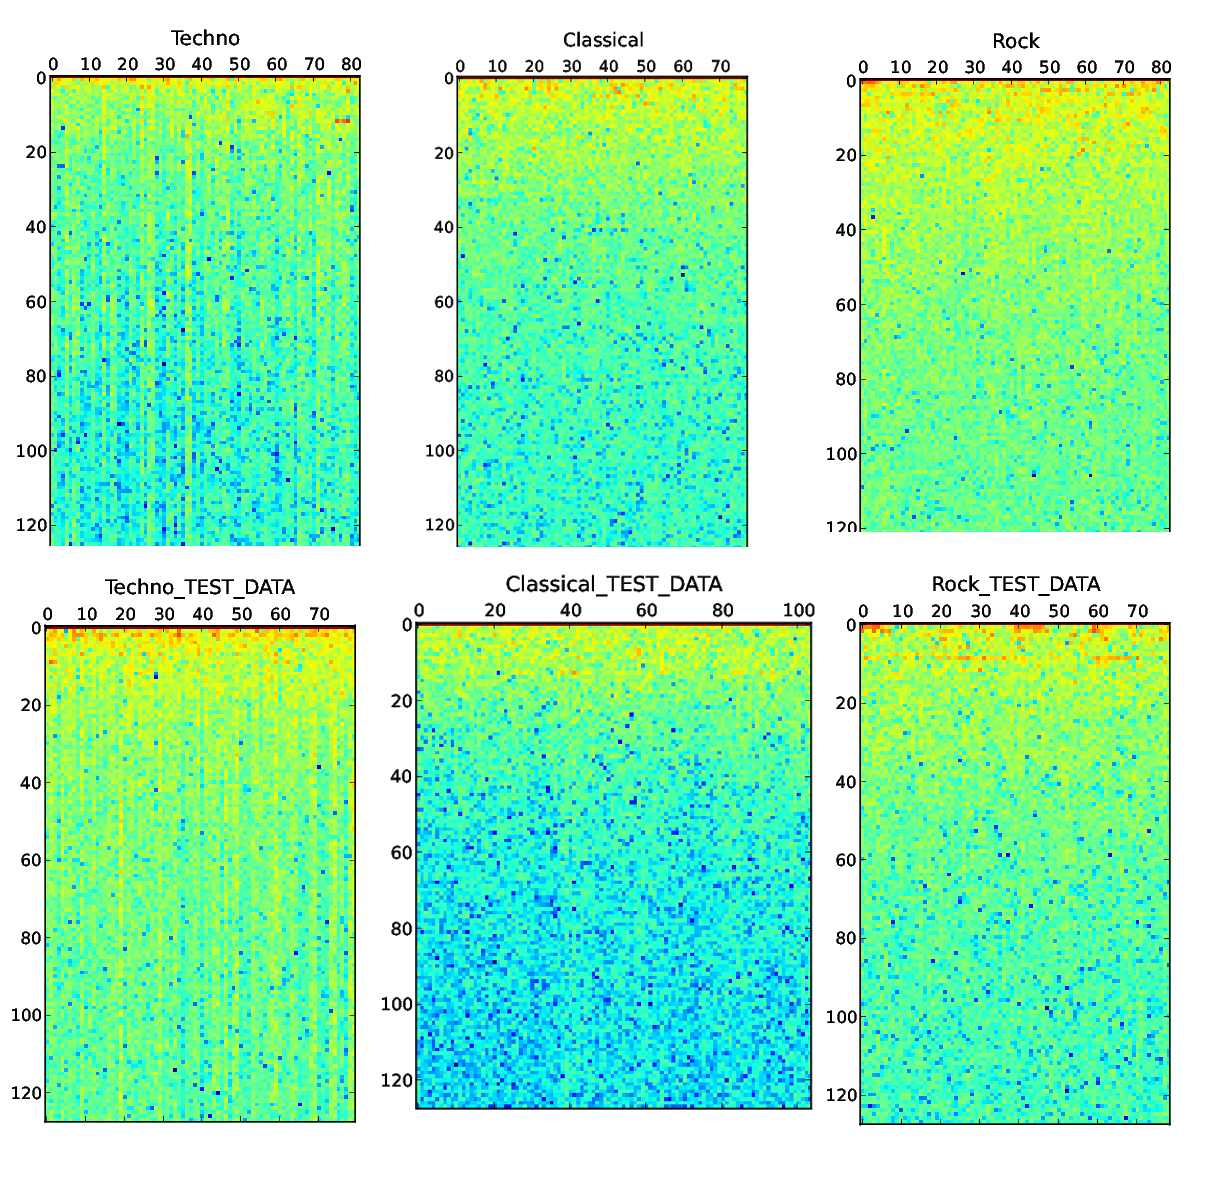
\includegraphics[scale=.2]{./all_ffts.png}
 % exp2_dataset.png: 813x175 pixel, 72dpi, 28.68x6.17 cm, bb=0 0 813 175
\end{center}
\caption{Spectrograms of Input Data For Audio Classification}
\label{fig:FFTS}
\end{figure}

The ``Training'' tag indicates that the network was exposed to sequential samples of that song's
FFTs in entirety, and then shown random 1 second clips from the spectrogram in rotation with the
other Training songs. ``Testing'' songs were never exposed to the network during the training
phase, but during the classification stage the HQSOM was asked to classify them. A network was built
that consisted of two base SOM-RSOM nodes that take in 64 inputs each (half of the 128) and each
output a BMU to a second SOM-RSOM, which then output their BMUs to a combined 2d vector which is
used as the input to a final SOM-RSOM node which outputs the classification BMU (See the attached
code for exact parameter details).  Unfortunately, the reference SOM-RSOM implementation was
entirely unable to separate the data, resulting in a 1-classifier for this network and every
other network that we could concieve of. When we used this network in conjunction with our
improvements, however, we were able to get the following positive results:
\begin{center}
\small
\begin{verbatim}
################################################################################
Results for Techno
Final Distribution Over Map Space
[ 0.265  0.349  0.     0.386  0.   ]
MODE: 3
################################################################################
Results for TechnoTEST
Final Distribution Over Map Space
[ 0.287  0.275  0.     0.438  0.   ]
MODE: 3
################################################################################
Results for Classical
Final Distribution Over Map Space
[ 0.526  0.154  0.     0.321  0.   ]
MODE: 0
################################################################################
Results for ClassicalTEST
Final Distribution Over Map Space
[ 0.49   0.202  0.     0.308  0.   ]
MODE: 0
################################################################################
Results for Rock
Final Distribution Over Map Space
[ 0.434  0.554  0.     0.012  0.   ]
MODE: 1
################################################################################
Results for RockTEST
Final Distribution Over Map Space
[ 0.266  0.734  0.     0.     0.   ]
MODE: 1
\end{verbatim}
\end{center}

These are the results after cycling through each training song in its entirety, followed by three
random 1-second window exposures for each song, making sure to clear the HQSOM's difference matrix
when switching between songs.  From them, we observe that the network has successfully separated the
three different songs presented in the training data.  More impressively, however, it has also
successfully classified the out-of-sample data by genre, even though these data were not even taken
from the same songs as those in the training set.

We note that the differences between the activation levels of the BMUs for different genres in this
result were in some cases small, and thus that the network was close to misclassifying some of the
data.  We also note that it took quite a bit of parameter tweaking to obtain the above results. 
Given our limited time and computational resources, however, we consider this acceptable as a
proof-of-concept.

Using only a single training cycle, we have successfully applied an HQSOM network to form invariant
representations of the genres of three musical pieces.  Further, we have applied these
representations to correctly classify three additional songs to which the network had never been
previously exposed.  We did this with no hard-coded \em a priori \em knowledge whatsoever -- the
network obtained the sum total of its musical knowledge through exposure to a single play of each of
the respective training songs.

\section{Discussion and Conclusions}

HQSOMs represent a promising path towards invariant spatio-temporal reasoning through massively
parallel vector math. This paper has successfully reproduced many of the results of Miller and
Lommel, improved upon the convergence and noise tolerance properties of their algorithm, and
extended the HQSOM model into the audio domain where these types of networks show great promise. We
have demonstrated that HQSOMs can simultaneously perform spatial and temporal clustering at multiple
layers of abstraction, permitting invariant feature representation and classification over both
space and time. Further, we have shown that they can do so in the presence of considerable noise,
and that they perform quite robustly out of sample -- in particular, they can successfully classify
never-before-seen audio data according to the highly abstract criterion of genre. All of this is
done in a fully unsupervised fashion.

In performing our experiments, however, we have also identified a number of shortcomings in both the
original HQSOM model that persist in our improved version. We have found that the networks are
highly sensitive
to parameter values and to some extent initial conditions, and that they often exhibit problems with
premature convergence. We believe these issues present promising avenues for further research, with
a particular focus on automatically tuning system parameters based on descriptive metrics for the
input data and the sets of SOM and RSOM map units. This would effectively reduce the number of
parameters
requiring specification in the model, and would make network performance much less reliant on the 
empirical testing of configuration settings. As an example, the adaptive $\gamma$ as shown in this
paper is a good start, but these networks must become less fragile if they are to be widely adopted.

More broadly, our work has enabled us to characterize the essential properties of the general class
of hierarchical, invariant, spatiotemporal representation and classification algorithms. Namely,
they must perform recurrent spatial and temporal clustering over multiple levels of a hierarchy
while preserving the underlying topology of their high-dimensional input data. It has not escaped
our notice that SOMs are merely one of many topology-preserving techniques for nonlinear
dimensionality reduction, and we strongly believe that the use of others such as locally linear
embedding or Isomap in a sort of generalized spatiotemporal representation algorithm could yield
promising results.

The incorporation of feedback mechanisms sending information from higher regions to lower ones also
appears as an immediate possibility for extension, and including such capabilities would provide a
means for auto-associativity and prediction much like that attempted by the HTM model.\cite{HTMAlgo,
OnIntelligence} Having already
incorporated the property of invariance, there is considerable reason to believe that a generalized
spatiotemporal representation algorithm with such feedback could add emergence, reification, and
multistability to its repertoire, completing its implementation of the core principles of gestalt
systems.\cite{HTMAlgo, OnIntelligence} Much more distant possibilities include the incorporation of
reinforcement learning, models of motor control and attention, and the capacity for episodic memory
formation, with the eventual goal of constructing simulated or robotic intelligent agents that
exhibit goal-directed behaviors and learn from their interactions with the
world.\cite{OnIntelligence} For now, however, we are pleased with our results and look forward to
further investigation.


\begin{thebibliography}{}


\bibitem{AIHistory1} M. Lungarella, F. Iida, J. C. Bongard, R. Pfeifer. \textsc{AI in the 21st
Century -- With Historical Reflections}. 50 Years of AI, Festschrift, LNAI 4850, pp. 1–8, 2007.


\bibitem{Rosenblatt} F. Rosenblatt. \textsc{The Perceptron: A Probabilistic Model for Information
Storage and Organization in the Brain}. Cornell Aeronautical Laboratory, Psychological Review, v65,
No. 6, pp. 386–408, 1958.


\bibitem{DreyfusMind} H. L. Dreyfus, S. E. Dreyfus. \textsc{Making a Mind versus Modeling the Brain:
Artificial Intelligence Back at a Branchpoint}. \em Daedalus \em, v117, No. 1, Artificial
Intelligence pp. 15–43, Winter, 1988.
\bibitem{AIHistory2} J. Schmidhuber. \textsc{AI in the 21st Century -- With Historical Reflections}.
50 Years of AI, Festschrift, LNAI 4850, pp. 29–41, 2007.


\bibitem{MLHistory1} J. G. Carbonell, R. S. Michalski, T. M. Mitchell. \textsc{Machine Learning: A
Historical and Methodological Analysis}. The AI Magazine, pp. 69–79, Fall 1983.


\bibitem{Poggio} T. Serre, M. Kouh, C. Cadieu, U. Knoblich, G. Kreiman, T. Poggio. \textsc{A Theory
of Object Recognition: Computations and Circuits in the Feedforward Path of the Ventral Stream in
Primate Visual Cortex}. AI Memo 2005-036. CBCL Memo 259. Massachusetts Institute of Technology,
Center for Biological and Computational Learning. Dec. 2005.


\bibitem{HQSOM} J. W. Miller and P. H. Lommel. \textsc{Biomimetic sensory abstraction using
hierarchical quilted self-organizing maps}. The Charles Stark Draper Laboratory, Inc. 555 Technology
Square, Cambridge, MA 02139-3563, USA. 2006.
\bibitem{OnIntelligence} J. Hawkins and S. Blakeslee. \textsc{On Intelligence}. Tomes Books, Holt,
New York, USA. 2002.


\bibitem{HTMAlgo} J. Hawkings, S. Ahmad, D. Dubinsky. \textsc{Hierarchical Temporal Memory including
HTM Cortical Learning Algorithms}. Numenta, Inc. 811 Hamilton St., Redwood City, CA 94063, USA.
Sept. 2011.


\end{thebibliography}
\end{document}
